% Introduction

% ??? NEED block diagram of go()! check map? scan: yes/no? save map, move etc. (use that online code to block diagram tool)
% ??? Descripe framework in a section (see gdocs for input to block diagram) (or present at exam)
% ??? Mention we chose to focus on making our own code with the least use of finished libraries as possible, no error handling 
% ??? Mention the report will explain important aspects of out work and theoretical parts, 
%     while the finished product is a prototype and the code in the appendix
% 

% Problem / introduction?:
% - Problem and analysis:
% 	- https://en.wikipedia.org/wiki/Rescue_robot
%	- https://www.robocupgermanopen.de/sites/default/files/rescue_maze_2017.pdf
% - System diagram (what we want to build):
% Daniel has already made a nice diagram of this
% Current position should be known after each move.

% - Prototype / mechanical design / robot design (show what we wanted to to build)
% - maybe here with motor/wheels under it? chasis?
% - maybe under "problem and analysis"


% Programming Structure and Design: (try to fulfill some Akbar goals here, see those gdocs notes)
%- Robot Instruction Execution Order
%- Framework
%- Data Structure



% Robot control: (maybe after pathfinding?)
% Theory:
% - functionality
% - step/control sequence
% Implementation: (programming)
% - programming/framework etc.

% Map handling:
% Theory (how we did and thoughts):
% - Introduction (what is map handling about, what have we covered here, problems we want to solve)
% - Analysis of map input
% - Converting analog map to digital map (intro)
% - 
% Implementation:
% - Read, compare, update 

% Prototype:
% maybe something about the prototype here??
% or in conclusion at least
% read google docs



\chapter{Map Handling}
\label{ch:map_handling} % chapter label
The rescue robot should be able follow a given path from start to finish, based on a predefined map given as input.
A map provides useful information about whether areas of the map are accessible or not. Map data can be loaded by the robot prior to its physical presence at a location. Once the robot is at the starting point, it has to rely on its sensors for updated information about the surroundings. 

The map itself is a crucial part, that converted into to a graph is used by the path-finding as explained in Chapter \ref{ch:path}. Hence a structured way of storing the required map data for different maps was designed. The primary goal was make it readable by the microcontroller, but also still allow easy user input.

%Existing pathfinding algorithms such as Dijkstra and A* was studied, 
%in order to understand what input data such algorithms typically would require. 
%The pathfinding algorihtm implemented in this project is further described in chapter \ref{ch:path}.

\newpage
\section{Map Requirements}
\label{sec:map_requirements}
Maps can be found in a lot of different styles,
varying in how they represent specific informations.
Those styles often depend on the purpose of the map.
Figure \ref{sub:orient} shows a map for casual orientation purposes,
while \ref{sub:evac} shows a standardized evacuation plan.

\begin{figure}[h!tp]
    \centering
    \subfloat[Section of AAU Esbjerg]{%
        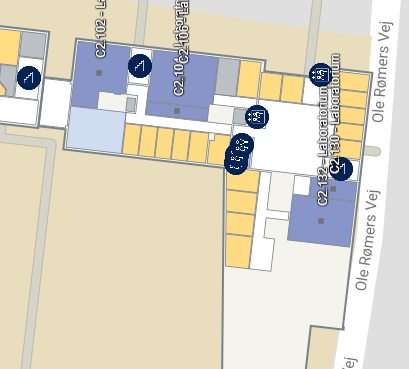
\includegraphics[width=0.4\textwidth]{figures/map/floorplan_aau.png}%
        \label{sub:orient}
        }%
    \hspace{0.1\textwidth}
    \subfloat[School layout example]{%
        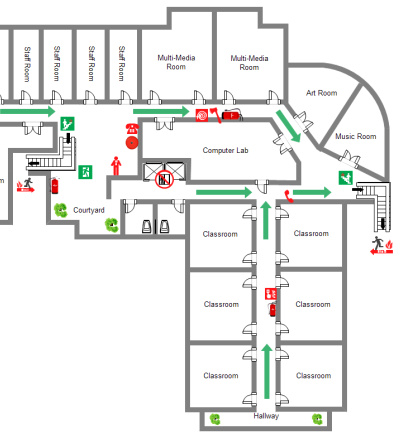
\includegraphics[width=0.4\textwidth]{figures/map/floorplan_school.png}%
        \label{sub:evac}
        }%
    \caption{Examples of different maps}
    \label{fig:floor_plans}
\end{figure}
% https://www.edrawsoft.com/school-layout-example.php

Maps are often very visual, providing a lot of detailed information to the reader.
The way the information is represented differently,
makes it very hard to be interpreted automatically.
A map must provide necessary information,
in a way that can be interpreted by the micro controller.
For this project we decided that a simplified map, would be sufficient.

Table \ref{table:map_data} shows the data the map should include,
as well as some areas that have been delimited from.

\begin{table}[h!]
	\centering
	\caption{Map data}
	\begin{tabular}{|p{0.4\textwidth}||p{0.4\textwidth}|}
		\hline
		Data to be included & Data to delimit from \\ 
		\hline
		Map dimensions 		& \parbox[t]{0.4\textwidth}{Differences in height\\(levels, stairs etc.)}\\
		\hline
		Start position 		& Door openings \\
		\hline
		Finish position 	& \parbox[t]{0.4\textwidth}{Ground surface\\(slipping, traction)} \\
		\hline
		Walls 				& Objects\\
		\hline
	\end{tabular}
	\label{table:map_data}
\end{table}


\section{Map Coordinates}
\label{sec:map_coordinates} % section label
During the theoretical development we often used hand-drawn 2D maps with grids as depicted in Figure \ref{sub:2d_map}. The map can have a certain size and allows for an object to have a location on the grid. A specific part of the map can easily be referred to by its unique coordinate in the x and y dimensions. 

For converting and storing analog maps into a usable digital representation with the same properties, we chose to use 2D arrays as data structure. A 2D array can be thought of as a matrix, where a grid of numbers can be arranged in rows and columns. 2D arrays are very similar to matrices, and differs in how elements are indexed.

The result of the different indexing methods can be seen by comparing Figure \ref{sub:2d_map} to \ref{sub:2d_array}. Given the same index values, the cell referred to would be different, as seen in  Figure \ref{sub:2d_map} and \ref{sub:2d_array}.

\begin{figure}[htp]
    \centering
    \subfloat[2D grid map]{%
        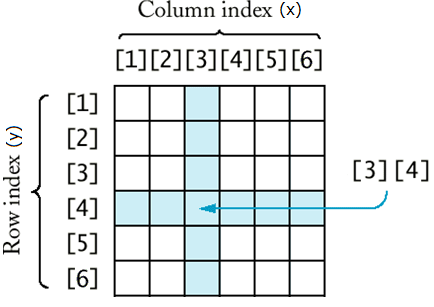
\includegraphics[width=0.45\textwidth]{figures/map/2d-map.png}%
        \label{sub:2d_map}
        }%  
    \hspace{0.05\textwidth}  
    \subfloat[2D array]{%
        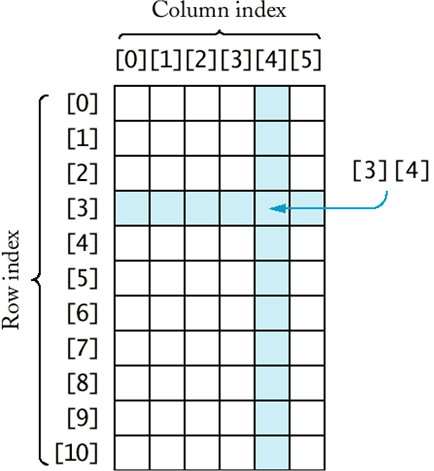
\includegraphics[width=0.45\textwidth]{figures/map/2d-array.png}%
        \label{sub:2d_array}
        }%
    \caption{Difference in indexing for (3,4) in a 2D grid map and a 2D array}
    \label{fig:floor_plans}
\end{figure}
%https://i.stack.imgur.com/tFdLk.gif

Each cell in the map represents a map segment with its own coordinate. To allow for a more logical access to segments of the map in the actual programming, we chose to start map coordinates at zero. Rows and columns could be switched when needed. This could be either be done in the syntax, by switching i and j, or by switching the x and y axes when storing the map in the first place.
\\

Example of map segment before rows and columns are switched
\begin{lstlisting}[language=Python]
Array: map[4][3], would give map coordinate (3,4)
\end{lstlisting}

Example of map segment after switching rows and columns
\begin{lstlisting}[language=Python]
Array: map[3][4], would give map coordinate (3,4)
\end{lstlisting}

This lead to the final implementation in our program using 2D arrays, 
where the value of any given map segment easily could be accessed. 
\\
Example of implementation in the final code
\begin{lstlisting}[language=Python]
Array: robot->map->segments[3][4], would return the value for map coordinate (3,4)
\end{lstlisting}
Examples of this can be seen implemented in the final code in appendix XX (some specific place?). 
\todo{fix referring to code in appendix, and code language should not be set to Python.} 
The same approach was used for handling node maps, which is further explained in Chapter \ref{ch:path}.


\section{Map Design}
\label{sec:map_design} % section label
The grid-based map is made up of simple plain-text ASCII characters. 
This makes it fairly simple and easy-to-understand, and maps can easily be created or changed by a user. An example of a 5x5 map can be seen in Figure \ref{sub:map_ascii}, where \# being walls, A being the start, B being the finish, o being nodes, and the white spaces being open spaces. Maps where also created using the UTF8 character encoding, which has a more characters to choose from, see Figure \ref{sub:map_utf8}.

Nodes represent positions on the map where the robot can move between. The idea is to allow movement in 8 directions, 4 straight and 4 diagonal, unless a direction is blocked by a wall. Nodes are explained further in Chapter \ref{ch:path}.


\begin{figure}[htp]
    \centering
    \subfloat[ASCII]{%
        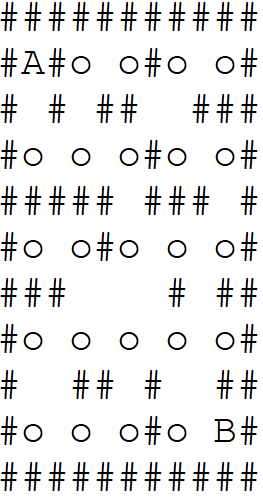
\includegraphics[width=0.2\textwidth]{figures/map/5x5map_ascii-2.png}%
        \label{sub:map_ascii}

    }
    \hspace{0.2\textwidth}
    \subfloat[UTF8]{%
        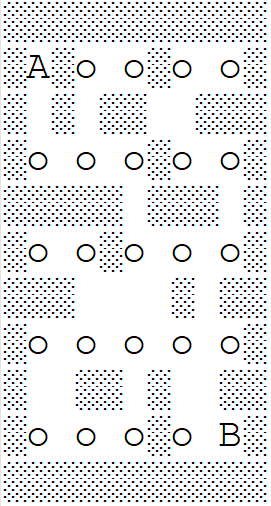
\includegraphics[width=0.2\textwidth]{figures/map/5x5map_utf8-2.png}%
        \label{sub:map_utf8}
    }
    \caption{5x5 map}
    \label{fig:5x5map}
\end{figure}

We found that UTF8 would require a bit more work, since text editors often add characters to the beginning of the file. 
This is known as the byte-order-mark (BOM) which indicates the file uses UTF8 encoding. 
It also uses variable bit-length for characters, between 1-4 bytes [https://en.wikipedia.org/wiki/UTF-8]. 
This makes reading and storing the map to a file more complicated, which is why we chose to use plain text ASCII.

\section{Reading map from input file}
\label{sec:map_read} % section label
In the C programming language the dimensions of an array must be declared at compile time. 
In this case, the array has to be large enough to hold all the map data. Unfortunately the map size and data remains unknown until a map is loaded at runtime.

The first idea was to use a fixed array large enough to hold maps of a predefined size. 
On the other hand, we thought this was as an excellent opportunity to try and work with pointers and dynamic memory allocation.

The required size of the array can be calculated by counting the lines and characters of the map, which is equivalent to the rows and columns. For a map with 5x5 nodes, there will be 11 characters in each line and a total of 11 lines.
To store the values an 11x11 2D array is required.\\
\\
Bunch of code could be inserted here\\
\\
- open file and read content\\
- count map size (rows and cols)\\
- allocating 2d array\\
- saving data in 2d array\\
- saving start and finish position

\section{Check Map}
\label{sec:map_check} % section label
Remember we have a chapter dedicated to scan.\linebreak
Based on scenario things might have dramatically changed, 
even to the point of map being useless or no map at all. 
Explain how map is updated.

\section{Map Save}
\label{sec:map_save} % section label

\section{Walls / Neighbours hex}
\label{sec:map_hex} % section label
Maybe this should be part of map check

\section{Node Map}
\label{sec:map_node} % section label



